\documentclass{beamer}
\usetheme{CWRU}

\title{Exploring Alternative Routes Using Multipath TCP}
\author{Stephen Brennan}
\date{June 5, 2017}

\usepackage{appendixnumberbeamer}
\usepackage{pgfpages}
\usepackage{wrapfig}
\usepackage{graphicx}
\setbeamertemplate{note page}[plain]
\setbeameroption{show notes on second screen=right}

\begin{document}
\frame{\titlepage}

\section{Introduction \& Background}

\begin{frame}
  \frametitle{Internet Routing Inefficiencies}
  \begin{columns}
  \begin{column}{0.7\textwidth}
  \begin{itemize}
  \item The default route is not always the best, in terms of latency or
    reliability
  \item Peering agreements and policy based routing can result in suboptimal
    routing decisions \cite{detour}
  \end{itemize}
  \end{column}
  \begin{column}{0.3\textwidth}
    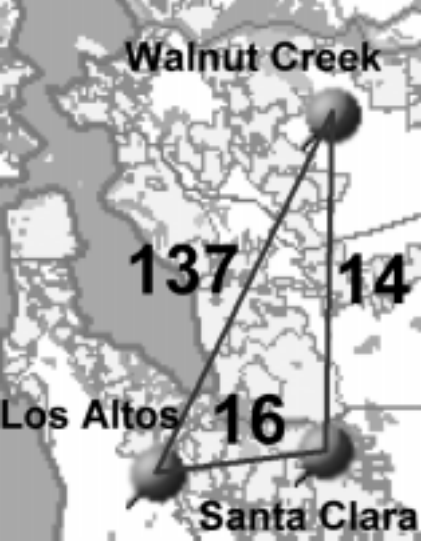
\includegraphics[width=\textwidth]{figures/detour.png} \\
    \textit{Figure from \cite{detour}}
  \end{column}
  \end{columns}
\end{frame}

\begin{frame}
  \frametitle{Internet Routing Inefficiencies}

  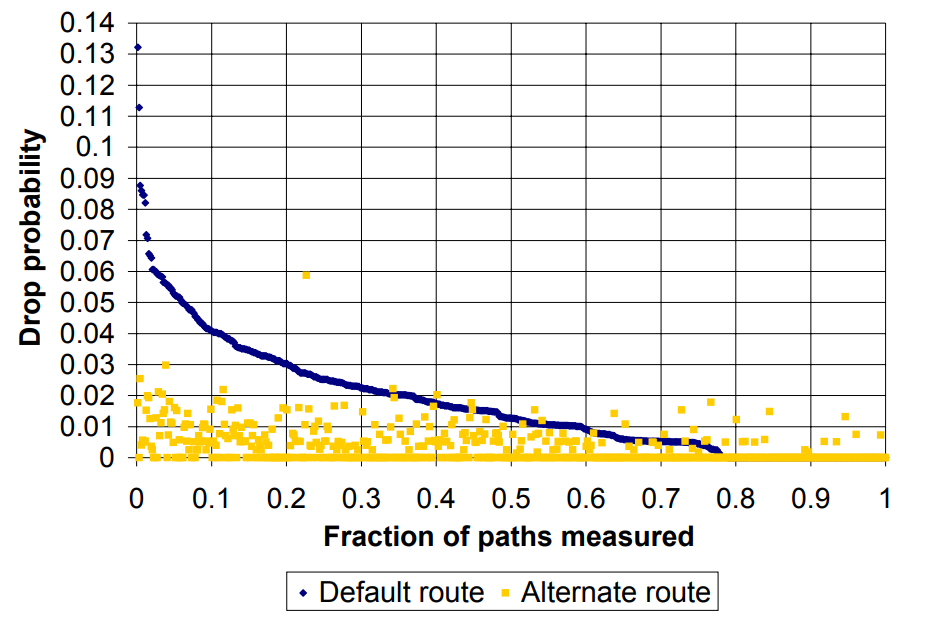
\includegraphics[height=0.85\textheight]{figures/detour-packetloss.png} \\
  \textit{Figure from \cite{detour}}
  \note{hello, world}
\end{frame}

\section{Related Work}
\section{Implementation}
\section{Evaluation}
\section{Conclusion}

\appendix % slide numbering includes nothing after here

\section{References}
\begin{frame}[allowframebreaks]
  \frametitle{References}
  \bibliographystyle{ieeetr}
  \bibliography{paper.bib}
\end{frame}

\end{document}